% Section content template for individual Educative lessons
% This file contains the actual content for a specific section
% Generated from Educative API section content

% Section: Background of Distributed Cache
% Section ID: 5353674067148800
% Section Slug: background-of-distributed-cache
% Generated: 2025-12-07T18:51:35.723741

The main goal of this chapter is to design a distributed cache. To achieve this goal, we should have substantial background knowledge, mainly on different reading and writing techniques. This lesson will help us build that background knowledge. Let's look at the structure of this lesson in the table below

\begin{table}[htbp]
\centering
\small
\adjustbox{max width=\textwidth}{
\begin{tabular}{|p{0.206\textwidth}|p{0.744\textwidth}|}
\hline
Section & Motivation \\
\hline
\hline
Writing policies & Data is written to cache and databases. The order in which data writing happens has performance implications. We'll discuss various writing policies to help decide which writing policy would be suitable for the distributed cache we want to design. \\
\hline
Eviction policies & Since the cache is built on limited storage (RAM), we ideally want to keep the most frequently accessed data in the cache. Therefore, we'll discuss different eviction policies to replace less frequently accessed data with most frequently accessed data. \\
\hline
Cache invalidation & Certain cached data may get outdated. We'll discuss different invalidation methods to remove stale or outdated entries from the cache in this section. \\
\hline
Storage mechanism & A distributed storage has many servers. We'll discuss important design considerations, such as which cache entry should be stored in which server and what data structure to use for storage. \\
\hline
Cache client & A cache server stores cache entries, but a cache client calls the cache server to request data. We'll discuss the details of a cache client library in this section. \\
\hline
\end{tabular}
}
\end{table}

\subsection{Writing policies}\label{pMnok9_dwrtG22EeBP7p4}
\\
Often, a cache stores a copy (or part) of data, which is persistently stored in a data store. When we store data to the data store, some important questions arise:
\begin{quote}
\begin{itemize}
\item
Where do we store the data first? Database or cache?
\item
What will be the implication of each strategy for consistency models?
\end{itemize}
\end{quote}
\\
The short answer is, it depends on the application requirements. Let 's look at the details of different writing policies to understand the concept better:

\begin{itemize}
\item
\protect\phantomsection\label{8rM2bjYtG6LiYIe1Cq9uE}
\textbf{Write-through cache}: The write-through mechanism writes on the cache as well as on the database. Writing on both storages can happen concurrently or one after the other. This increases the write latency but ensures strong consistency between the database and the cache.
\item
\protect\phantomsection\label{IQnxTkJX6KtFJoMOfu6Cp}
\textbf{Write-back cache}: In the write-back cache mechanism, the data is first written to the cache and asynchronously written to the database. Although the cache has updated data, inconsistency is inevitable in scenarios where a client reads stale data from the database. However, systems using this strategy will have small writing latency.
\item
\protect\phantomsection\label{u9LRu9pbPTsxswvgN1NFU}
\textbf{Write-around cache}: This strategy involves writing data to the database only. Later, when a read is triggered for the data, it's written to cache after a cache miss. The database will have updated data, but such a strategy isn't favorable for reading recently updated data.
\end{itemize}

\subsection*{Quiz}
\vspace{0.3cm}
\noindent
\textbf{Question 1:} A system wants to write data and promptly read it back. At the same time, we want consistency between the cache and database. Which writing policy is the optimal choice?
\\[0.2cm]
\begin{itemize}
 \item \textbf{[CORRECT]} Write-through cache
\\[0.1cm]
\textit{Explanation:} 
Reading will be prompt and data will be consistent in the database as well.
 \item Write-around cache
\\[0.1cm]
\textit{Explanation:} 
This choice will reduce performance because reading every recently written data entry will result in a cache miss.
 \item Write-back cache
\\[0.1cm]
\textit{Explanation:} 
Inconsistency may arise because data is written asynchronously to the source of truth (database).
\end{itemize}
\vspace{0.3cm}
\noindent
\textbf{Question 2:} With reference to performance, what should a write-heavy system avoid?
\\[0.2cm]
\begin{itemize}
 \item Write-back cache
\\[0.1cm]
\textit{Explanation:} 
This has the best performance because data is only written to the cache and after that written asynchronously to the database.
 \item \textbf{[CORRECT]} Write-through cache
\\[0.1cm]
\textit{Explanation:} 
Write-through cache has high write latency because it writes to the database as well as cache.
 \item Write-around cache
\\[0.1cm]
\textit{Explanation:} 
This is also bad because data is written to the database. However, write-around cache latency will be lower than that of write-through cache because the write-through writes to the database and the cache.
\end{itemize}
\vspace{0.3cm}
\noindent
\textbf{Question 3:} Which write policy typically leads to outdated or stale data when reading from the cache?
\\
\textit{(Select all that apply.)}
\\[0.2cm]
\begin{itemize}
 \item Write-through
 \item \textbf{[CORRECT]} Write-back
\\[0.1cm]
\textit{Explanation:} 
Because data is written asynchronously to the database.
 \item \textbf{[CORRECT]} Write-around
\\[0.1cm]
\textit{Explanation:} 
Because it bypasses the cache for write operations, leading to the possibility of data being quickly evicted from the cache before it's read again.
\end{itemize}

\subsection{Eviction policies}\label{-Y0s22qyaH2PfjjxqlSPL}
\\
One of the main reasons caches perform fast is that they're small. Small caches mean limited storage capacity. Therefore, we need an eviction mechanism to remove less frequently accessed data from the cache.\\
\strut \\
Several well-known strategies are used to evict data from the cache. The most well-known strategies include the following:

\begin{itemize}
\item
\protect\phantomsection\label{ySX_074h-xgqRlE7E6pKH}
Least recently used (LRU)
\item
\protect\phantomsection\label{dibt4_qtOXs62av3JSIMm}
Most recently used (MRU)
\item
\protect\phantomsection\label{qOR22YXehr7upRcZQOUHL}
Least frequently used (LFU)
\item
\protect\phantomsection\label{iF9dLR_SjNDWvamO1THVM}
Most frequently used (MFU)
\end{itemize}
\\
Other strategies like first in, first out (FIFO) also exist. The choice of each of these algorithms depends on the system the cache is being developed for.

\subsection{Cache invalidation}\label{bY-jXZXUUXz1waRCNhuly}
\\
Apart from the eviction of less frequently accessed data, some data residing in the cache may become stale or outdated over time. Such cache entries are invalid and must be marked for deletion.
\\
The situation demands a question: How do we identify stale entries?
\\
Resolution of the problem requires storing metadata corresponding to each cache entry. Specifically , maintaining a time-to-live (TTL)(TTL is the time after which a cache entry is considered expired.) value to deal with outdated cache items.
\\
We can use two different approaches to deal with outdated items using TTL:

\begin{itemize}
\item
\protect\phantomsection\label{yZepxwsJ51R_woGdGpTpd}
\textbf{Active expiration}: This method actively checks the TTL of cache entries through a daemon process or thread.
\item
\protect\phantomsection\label{R7gIIGSHeRhOK19-x7ZMl}
\textbf{Passive expiration}: This method checks the TTL of a cache entry at the time of access.
\end{itemize}
\\
Each expired item is removed from the cache upon discovery.

\subsection{Storage mechanism}\label{nGlGaNp5StJXUhen_u8WE}
\\
Storing data in the cache isn't as trivial as it seems because the distributed cache has multiple cache servers. When we use multiple cache servers, the following design questions need to be answered:

\begin{itemize}
\item
\protect\phantomsection\label{Brg6eYrXM2Njzqxgq__Va}
Which data should we store in which cache servers?
\item
\protect\phantomsection\label{xOJ7p1DIphR24B1f0_fP0}
What data structure should we use to store the data?
\end{itemize}
\\
The above two questions are important design issues because they'll decide the performance of our distributed cache, which is our most important requirement. We 'll use the following techniques to answer the questions above.

\subsubsection{Hash function}\label{uYoSThURzBVM8Qh-Y7yDl}
\\
It's possible to use hashing in two different scenarios:

\begin{itemize}
\item
\protect\phantomsection\label{hkbdlrWkEdLmlvWdPDEC0}
Identify the cache server in a distributed cache to store and retrieve data.
\item
\protect\phantomsection\label{7EMTE2GCEpB2P1WbMSAvl}
Locate cache entries inside each cache server.
\end{itemize}
\\
For the first scenario, we can use different hashing algorithms. However, consistent hashing or its flavors usually perform well in distributed systems because simple hashing won't be ideal in case of crashes or scaling.
\\
In the second scenario, we can use typical hash functions to locate a cache entry to read or write inside a cache server. However, a hash function alone can only locate a cache entry. It doesn't say anything about managing data within the cache server. That is, it doesn't say anything about how to implement a strategy to evict less frequently accessed data from the cache server. It also doesn't say anything about what data structures are used to store the data within the cache servers. This is exactly the second design question of the storage mechanism. Let's take a look at the data structure next.
\\
Explain why consistent hashing is preferred over simple hashing in distributed cache systems and how it improves scalability and fault tolerance.\\
\\
Use the AI assessment widget below to submit your solution and get an interactive response.

\textbf{Question:}

Why do we prefer consistent hashing?

\textbf{Reference Answer:}

Consistent hashing is preferred over simple hashing in distributed cache systems because it minimizes data movement when nodes are added or removed, improving scalability. It also enhances fault tolerance, as only a small portion of data needs to be redistributed when a node fails.

\subsubsection{Linked list}\label{Kc82fdY1KXVrA27xF30V8}
\\
We'll use a doubly linked list. The main reason is its widespread usage and simplicity. Furthermore , adding and removing data from the doubly linked list in our case will be a constant time operation. This is because we either evict a specific entry from the tail of the linked list or relocate an entry to the head of the doubly linked list. Therefore, no iterations are required.
\begin{quote}
\textbf{Note:} \href{https://www.educative.io/answers/what-is-a-bloom-filter}{Bloom filters} are an interesting choice for quickly finding if a cache entry doesn't exist in the cache servers. We can use bloom filters to determine that a cache entry is definitely not present in the cache server, but the possibility of its presence is probabilistic. Bloom filters are quite useful in large caching or database systems.
\end{quote}
\subsection{Sharding in cache clusters}\label{Q98c5DXwz9jazDvkvPVLg}
\\
To avoid SPOF and high load on a single cache instance, we introduce sharding. Sharding involves splitting up cache data among multiple cache servers. It can be performed in the following two ways.

\subsubsection{Dedicated cache servers}\label{PXXoauu5aDWmi_DSg9OFM}
\\
In the \textbf{dedicated cache servers} method, we separate the application and web servers from the cache servers.
\\
The advantages of using dedicated cache servers are the following:

\begin{itemize}
\item
\protect\phantomsection\label{HPEsTVsfn9tAWaEwjNnCq}
There's flexibility in terms of hardware choices for each functionality.
\item
\protect\phantomsection\label{WWHzNYce_ped_vpyQRdB9}
It's possible to scale web/application servers and cache servers separately.
\end{itemize}
\\
Apart from the advantages above, working as a standalone caching service enables other microservices to benefit from them---for example, Cache as a Service. In that case, the caching system will have to be aware of different applications so that their data doesn't collide.

Data can be classified into three temperature regions depending on the access frequency: - \textbf{Hot}: This is highly accessed data. - \textbf{Warm}: This is less frequently accessed data. - \textbf{Cold}: This is rarely accessed data.
\\
Cold data frequently gets evicted from the cache and gets replaced with hot or warm data. The following image shows the spectrum of data temperatures:

\begin{figure}[htbp]
 \centering
 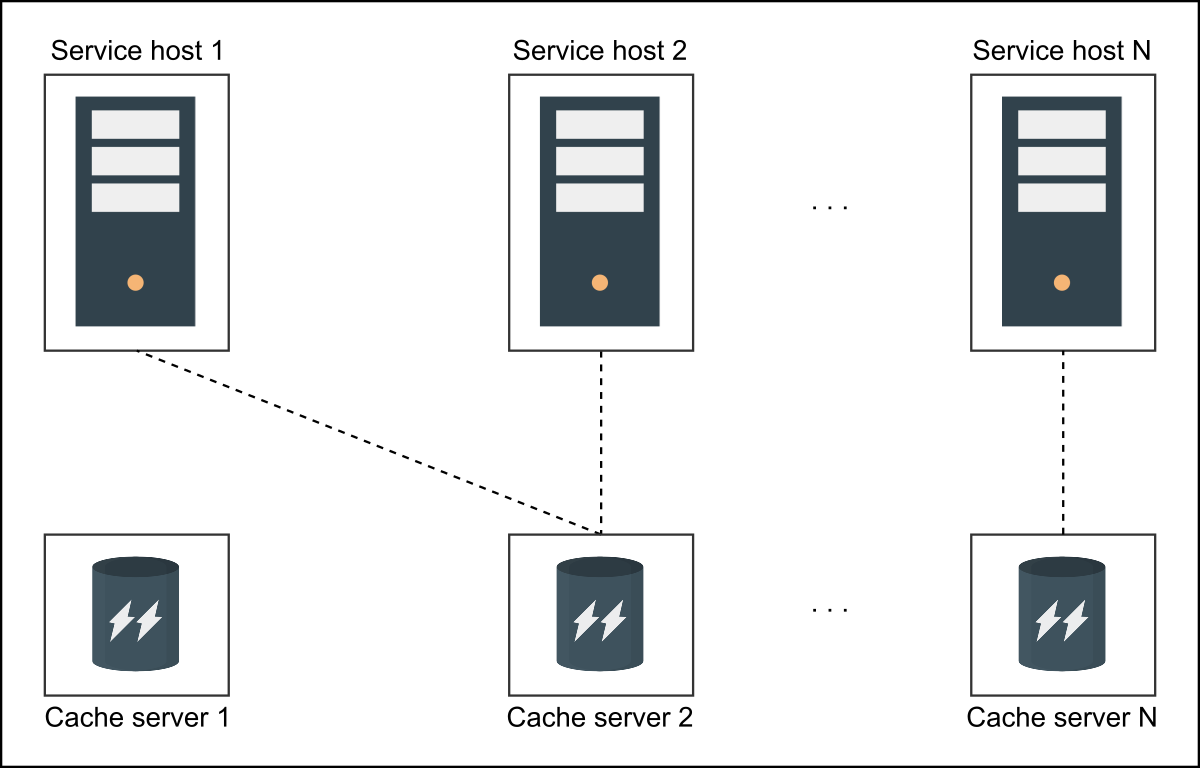
\includegraphics[width=0.25\textwidth]{Images/chapter_16/section_5353674067148800/6016998068977664.png}
 \caption{A depiction of service hosts coordinating with dedicated cache servers}
\end{figure}

\subsubsection{Co-located cache}\label{8s8io4aoNPWYotQ-SE6yJ}
\\
The co-located cache embeds cache and service functionality within the same host.
\\
The main advantage of this strategy is the reduction in CAPEX(Capital expenditures are major investments over assets that are held for a long time.) and OPEX(Operational Expenditures are day-to-day expenses that keep the company running.) of extra hardware. Furthermore , with the scaling of one service, automatic scaling of the other service is obtained. However, the failure of one machine will result in the loss of both services simultaneously.

\begin{figure}[htbp]
 \centering
 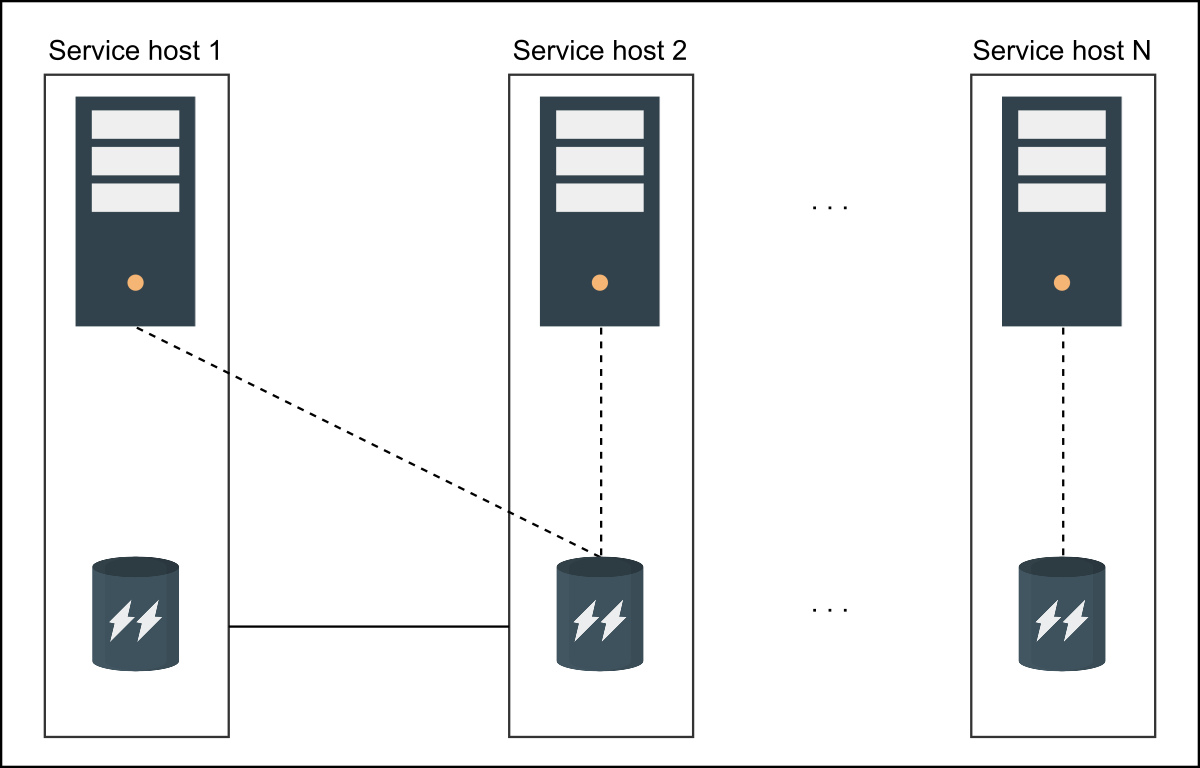
\includegraphics[width=0.25\textwidth]{Images/chapter_16/section_5353674067148800/4767542396846080.png}
 \caption{Hosting cache and application logic in the same machine}
\end{figure}

\subsection{Cache client}\label{lHas71PRXsmH13scItqXR}
\\
We discussed that the hash functions should be used for the selection of cache servers. But what entity performs these hash calculations?
\\
A cache client is a piece of code residing in hosting servers that do (hash) computations to store and retrieve data in the cache servers. Also , cache clients may coordinate with other system components like monitoring and configuration services. All cache clients are programmed in the same way so that the same PUT(Adding data to a cache server.), and GET(Retrieving data from a cache server.) operations from different clients return the same results. Some of the characteristics of cache clients are the following:

\begin{itemize}
\item
\protect\phantomsection\label{GrRhqb6U_9ZQHn-dp8eXK}
Each cache client will know about all the cache servers.
\item
\protect\phantomsection\label{zbwccHo7P3LmexPzULrE5}
All clients can use well-known transport protocols like TCP or UDP to talk to the cache servers.
\end{itemize}

\begin{quote}
\textbf{Quiz:}
\textbf{Question 1:} What will be the behavior of cache clients to an access request if one of the cache servers is dead?
\textbf{Answer:} Since the data within the cache servers will no longer be available,

cache clients will mark that access request as a cache miss.
\end{quote}

\subsection{Conclusion}\label{cf8yOrpRwjVzhXXmQ2TuN}
\\
In this lesson, we learned what distributed caches are and highlighted their significance in distributed systems. We also discussed different storage and eviction mechanisms for caches. Caches are vital for any distributed system and are located at different points within the design of a system. It 's important to understand how distributed caches can be designed as part of a large system.

% End of section content